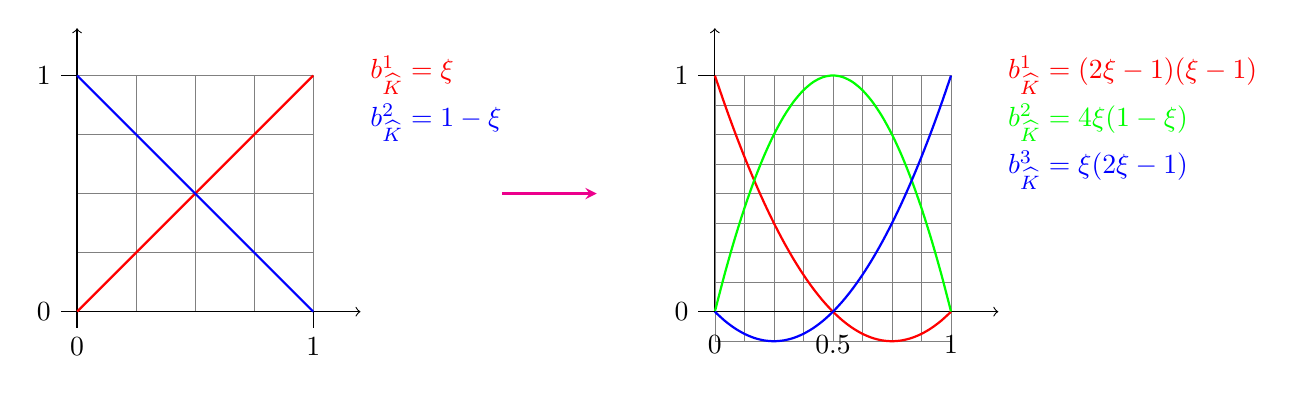
\begin{tikzpicture}[scale=3]
	\draw[step=.25cm,gray,very thin] (0,0) grid (1,1);		
	\draw[->] (0,0) -- (1.2,0);
	\draw[->] (0,0) -- (0,1.2);	
	
	\draw[domain=0:1,smooth,variable=\x,red,thick] 
		plot ({\x},{\x});
	\draw[domain=0:1,smooth,variable=\x,blue,thick] 
		plot ({\x},{1-\x});
	
	\draw (0,0)--(-.07,0) node [anchor=east] {0}
		(0,1)--(-.07,1) node[anchor=east] {1}
		(0,0)--(0,-.07) node [anchor=north] {0}
		(1,0)--(1,-.07) node[anchor=north] {1}
		(1.2,1) node[anchor=west,text=red] {$b_{\widehat{K}}^1=\xi$}
		(1.2,.8) node[anchor=west,text=blue] {$b_{\widehat{K}}^2=1-\xi$};
		
%	====================================================================	
	\draw [>=stealth,->,magenta,thick] (1.8,.5)--(2.2,.5);
%	====================================================================

	\draw[xshift=2.7cm,step=.125cm,gray,very thin] (0,-.125) grid (1,1);		
	\draw[xshift=2.7cm,->] (0,0) -- (1.2,0);
	\draw[xshift=2.7cm,->] (0,0) -- (0,1.2);	

	\draw[xshift=2.7cm,domain=0:1,smooth,variable=\x,red,thick] 
		plot ({\x},{(\x-1)*(2*\x-1)});	
	\draw[xshift=2.7cm,domain=0:1,smooth,variable=\x,green,thick] 
		plot ({\x},{4*\x*(1-\x)});
	\draw[xshift=2.7cm,domain=0:1,smooth,variable=\x,blue,thick] 
		plot ({\x},{\x*(2*\x-1)});
	
	\draw[xshift=2.7cm]
		(0,0)--(-.07,0) node [anchor=east] {0}
		(0,1)--(-.07,1) node[anchor=east] {1}
		(0,-.14) node {0} (.5,-.14) node {0.5} (1.,-.14) node {1}
		(1.2,1) node[anchor=west,text=red]{$b_{\widehat{K}}^1=(2\xi-1)(\xi-1)$}
		(1.2,.8) node[anchor=west,text=green]{$b_{\widehat{K}}^2=4\xi(1-\xi)$}
		(1.2,.6) node[anchor=west,text=blue]{$b_{\widehat{K}}^3=\xi(2\xi-1)$};	
\end{tikzpicture}

